\section{Sučelje prema percepciji}
\label{sec:sucelje-percepcija}

\subsection{Prijenos podataka između percepcije i upravljanja}
\label{subsec:udp-most}

Budući da se percepcijski cjevovod i upravljački sloj izvode u odvojenim izvedbenim okruženjima na istom računalu (poglavlje~\ref{ch:sustav}), potreban je most između njih. Percepcijska strana šalje UDP paket u JSON formatu, koji sadrži dvije vrijednosti (\texttt{px}, \texttt{py}), pikselnu poziciju ciljne točke zaokruženu na cijeli broj. Slanje obavlja jednostavna UDP utičnica (\emph{socket}) klase \texttt{UDPSender}, koja paket šalje na unaprijed zadanu IP adresu i port (5005) Docker okruženja pri svakoj sličici za koju postoji ciljna točka, bez potvrde primitka ili ponovnog slanja u slučaju gubitka paketa.

Na Docker strani, namjenski ROS čvor prima paket, popunjava poruku tipa \texttt{PointStamped} vrijednostima \texttt{point.x} i \texttt{point.y}, dok se \texttt{point.z} uvijek postavlja na nulu budući da sustav ne raspolaže mjerenjem udaljenosti do cilja, te je objavljuje na temu \texttt{ibvs/target\_point}, izvorno sučelje koje paket \texttt{ibvs\_perching} inače koristi s vlastitim (ArUco) modulom percepcije. Time se omogućuje da isti upravljački sloj prima ciljnu točku i od ArUco modula i od cjevovoda za detekciju grane, bez izmjena u samom upravljanju. Naredba za vertikalno kretanje ne izvodi se iz ove poruke, nego je unaprijed zadana konstanta u upravljačkom sloju (vidi Odjeljak~\ref{subsec:prijanjanje}).

\subsection{Preslikavanje osi za kameru okrenutu prema gore}
\label{subsec:preslikavanje-osi}

% TODO: ovo poglavlje dovrsiti nakon eksperimentalne provjere stvarnog predznaka i
% osi -- trenutno opisuje namjeravano ponasanje, ne izmjereno

Paket \texttt{ibvs\_perching} izvorno pretpostavlja kameru okrenutu prema dolje, gdje vodoravni pomak u slici odgovara pomaku unaprijed, a okomiti pomak pomaku ulijevo/udesno. U ovom radu, s kamerom okrenutom prema gore, vodoravni pomak u slici umjesto toga upravlja bočnim nagibom, a okomiti pomak nagibom naprijed-natrag, dok os prilaska (penjanje) preuzima ulogu koju je izvorno imao pomak unaprijed. Upravljački sloj ne koristi nikakav vanjski koordinatni sustav, nego se oslanja isključivo na vlastitu inercijsku/AHRS procjenu orijentacije letjelice, pa je preslikavanje osi jedina prilagodba potrebna za rad s kamerom okrenutom prema gore. Obje se osi pritom normaliziraju istom polovinom širine slike, a ne svaka svojom polovinom dimenzije, budući da bi dijeljenje okomite pogreške njezinom vlastitom, manjom polovinom visine slike isto pojačanje regulatora učinilo jačim na toj osi.

\section{Upravljačka petlja}
\label{sec:upravljacka-petlja}

Na strani upravljanja, Ji i sur.~\cite{ji2022realtimetrajectoryplanningaerial} predstavili su metodu planiranja trajektorije u stvarnom vremenu za zračno prijanjanje. Samadikhoshkho i Lipsett~\cite{drones8110605} kombinirali su duboko učenje s vizualnim navođenjem temeljenim na slici za zračno uzorkovanje vegetacije. Domišlović i sur.~\cite{domislovic_marsupial} demonstrirali su vizualno navođenje temeljeno na poziciji s marsupijalnim robotskim sustavom, pristup srodan onome korištenom u ovom radu. Kim i Chang~\cite{drones10040270} predstavili su sustav prijanjanja bez markera za kvadrokopter koji kombinira model segmentacije sa senzorom udaljenosti i upravljačem temeljenim na konačnom automatu, izvodeći cijeli cjevovod na Jetson Orin NX platformi. Do i Hong~\cite{do2023visionbased} ostvarili su vizualno prijanjanje nano letjelice na vodoravnu površinu korištenjem monokularne kamere i procjene poze u odnosu na oznaku. He i sur.~\cite{he2023imagebased} primijenili su vizualno navođenje temeljeno na slici za zračnu manipulaciju potpuno pokretljivom letjelicom, prateći linijske značajke umjesto točkastih. Mao i sur.~\cite{mao2023robust} razvili su robusno aktivno vizualno prijanjanje kvadrokoptera na nagnute površine uz ponovno planiranje putanje u stvarnom vremenu. Di i sur.~\cite{di2026slap} predstavili su sustav prijanjanja na okomita debla drveća koji kombinira vizualnu detekciju mjesta prijanjanja s IMU-temeljenom detekcijom neuspjelog pokušaja i mehanizmom oporavka. Za razliku od ovih pristupa, koji redom pretpostavljaju raspoloživ sustav apsolutne lokalizacije, senzor udaljenosti za okidanje prijanjanja ili poznatu oznaku/površinu cilja, upravljački sloj korišten u ovom radu ne oslanja se ni na jedno od toga.

Letjelicom upravlja paket \texttt{ibvs\_perching}~\cite{ibvs_perching}, izgrađen nad ArduPilot autopilotom i MAVROS mostom prema ROS-u~\cite{aliane2024survey}. Taj paket ne koristi kontroler pozicije niti vanjsku lokalizaciju: letjelicom upravlja izravno preko sučelja \texttt{mavros/setpoint\_raw/attitude}, šaljući ciljnu orijentaciju letjelice za bočno poravnanje (Odjeljak~\ref{subsec:pid-kaskada}) te naredbu brzine penjanja (kroz polje \texttt{thrust}, protumačeno u ArduPilot GUIDED načinu rada kao naredba brzine penjanja, a ne kao sirovi potisak) za okomiti prilazak.

\subsection{Kaskadni regulator položaja}
\label{subsec:pid-kaskada}

Vodoravno poravnanje ostvaruje se kaskadnom strukturom s dvije razine. Vanjska petlja preslikava normaliziranu pikselnu pogrešku u željeni nagib letjelice (\emph{tilt}) preko dva neovisna PID regulatora, jednog za svaku os. Pojačanje regulatora izraženo je u radijanima nagiba po jediničnoj pogrešci, tako da izlaz regulatora izravno predstavlja nagib koji se naređuje na rubu slike, a ne kutnu brzinu. Integralni član sprječava trajno odstupanje u prisutnosti stalnog poremećaja poput vjetra, dok derivacijski član, izračunat iz razlike uzastopnih detekcija, unaprijed koči prilazak i ublažava nadmašaj. Derivacijski član zanemaruje se ako je razmak između dvije uzastopne detekcije predugačak, budući da bi u tom slučaju izražavao stvarno pomicanje cilja, a ne brzinu njegova kretanja u odnosu na letjelicu.

\begin{figure}[htb]
\centering
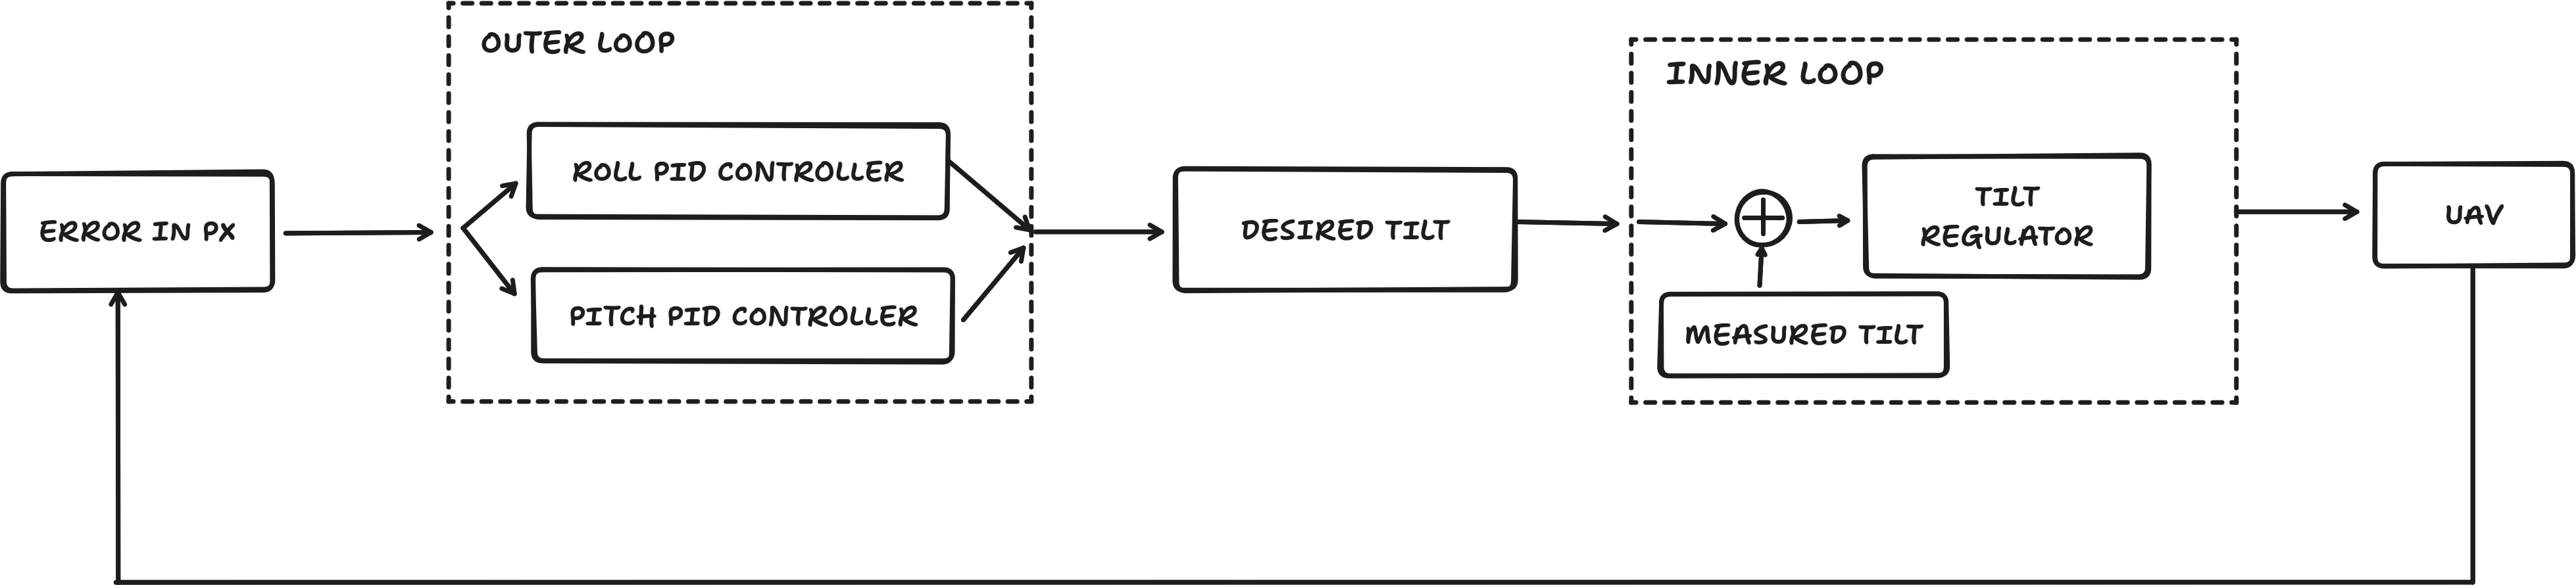
\includegraphics[width=1.0\textwidth]{images/cascade_controller.png}
\caption{Kaskadni regulator položaja: vanjska petlja (dva PID regulatora, po jedan za svaku os) preslikava pikselnu pogrešku u željeni nagib, koji se u \emph{attitude} načinu šalje kao ciljna orijentacija unutarnjoj petlji ArduPilota.}
\label{fig:cascade_controller}
\end{figure}

Izlaz vanjske petlje, željeni nagib, letjelici se predaje na jedan od dva načina, odabran postavkom upravljačkog sloja. U uobičajenom načinu (\emph{attitude}) željeni nagib šalje se izravno kao ciljna orijentacija (kvaternion), a unutarnju petlju koja tu orijentaciju pretvara u stvarnu kutnu brzinu zatvara sam ArduPilot, koristeći vlastite, tvornički ugođene regulacijske parametre pri visokoj frekvenciji. Alternativni način (\emph{rate}) šalje izravno naredbu kutne brzine tijela, izračunatu jednostavnim proporcionalnim regulatorom iz razlike između željenog i trenutnog nagiba, gdje se trenutni nagib očitava iz AHRS procjene orijentacije letjelice (poglavlje~\ref{sec:teorijska-podloga}). Ovaj se način koristi isključivo za usporedbu na klupi, dok se u letu koristi prvi način.

Izbor načina \emph{attitude} za let nije proizvoljan: raniji pokušaji leta u načinu \emph{rate} pokazali su da naredba nagiba u smjeru propinjanja (\emph{pitch}) zasićuje na graničnoj vrijednosti (\texttt{max\_tilt}) u velikoj većini uzoraka tijekom poravnanja, budući da jednostavan proporcionalni regulator kutne brzine, bez unutarnje petlje koju bi zatvarao autopilot, sporije i nestabilnije prati zadani nagib. Prelaskom na \emph{attitude} način, ArduPilotova vlastita, tvornički ugođena unutarnja petlja preuzima to zatvaranje pri znatno višoj frekvenciji, čime se zasićenje izbjeglo i let postao stabilniji. Neovisno o odabranom načinu, kruta veza između kamere i tijela letjelice unosi i fizičku vezanost između naređenog nagiba i same slike: svaki nagib koji regulator naredi istovremeno zakreće vidokrug kamere, što se u pikselnoj pogreški očituje kao kratkotrajan skok neposredno prije nego što stvarno translacijsko gibanje letjelice počne pogrešku smanjivati. Ova je vezanost svojstvena samoj geometriji sustava, a ne posljedica odabira načina slanja naredbe, i razmatra se i u poglavlju~\ref{ch:rezultati} na stvarnim podacima leta.

Naredba nagiba ograničena je unaprijed zadanom maksimalnom vrijednošću, neovisno o veličini pikselne pogreške. Ovo ograničenje ujedno predstavlja i glavnu sigurnosnu granicu sustava: bez obzira na to koliko velika pogreška u slikovnoj ravnini bude, ili kako pogrešno predznak preslikavanja osi bude postavljen, letjelica se ne može nagnuti strmije od ove granice, čime se ograničava i najveća moguća brzina vodoravnog pomicanja.

\subsection{Stanje sustava}
\label{subsec:state-machine}

Upravljački sloj strukturiran je kao konačni automat sa sedam stanja, koji određuje smije li se u danom trenutku uopće izvoditi poravnanje ili vertikalno kretanje. Letjelica polazi u stanju čekanja naoružavanja, u kojem se naredbe nagiba i penjanja drže na neutralnim vrijednostima (razina i lebdenje). Nakon što je letjelica naoružana i prebačena u odgovarajući način leta, sustav prelazi u stanje mirovanja ako cilj trenutno nije vidljiv, odnosno u stanje pripravnosti ako je cilj u tom trenutku vidljiv (potonje je isključivo informativna oznaka operateru da je poravnanje spremno početi). Servoiranje se aktivira zasebnim zahtjevom (uslugom), nakon čega sustav prelazi u stanje poravnanja te, kada pogreška padne ispod praga i ondje ostane dovoljno dugo, u stanje poravnano, u kojem se izvodi i vertikalno kretanje opisano u nastavku. Ako se cilj tijekom poravnanja ili nakon njega izgubi na razdoblje dulje od unaprijed određenog praga, sustav prelazi u stanje izgubljenog cilja, u kojem se letjelica vraća na razinu i miruje dok se cilj ponovno ne pojavi.

Izlazak iz stanja poravnano zahtijeva da pogreška premaši prag pomnožen histereznim faktorom, čime se sprječava treperenje između stanja poravnanja i poravnano oko same granice praga. Iz bilo kojeg stanja, gubitak naoružanja ili napuštanje odgovarajućeg načina leta letjelicu odmah vraća u stanje čekanja naoružavanja, neovisno o tome što se u tom trenutku događalo. Ova zaštita djeluje neovisno o softveru upravljačkog sloja: promjena načina leta obavlja se isključivo ručno, preko prekidača na daljinskom upravljaču sigurnosnog pilota, pa upravljački sloj nikada sam ne preuzima niti prepušta kontrolu nad letjelicom. Time sigurnosni pilot u svakom trenutku zadržava mogućnost trenutačnog preuzimanja ručnog upravljanja, neovisno o tome u kojem se stanju automat nalazi.

Sedam stanja u kodu nose nazive \texttt{WAIT\_ARM} (čekanje naoružavanja), \texttt{CLIMB} (penjanje pri uzlijetanju), \texttt{HOVER} (mirovanje), \texttt{TAG\_IN\_SIGHT} (pripravnost, cilj vidljiv), \texttt{ALIGN} (poravnanje), \texttt{ALIGNED} (poravnano) i \texttt{TAG\_LOST} (cilj izgubljen). Iz \texttt{WAIT\_ARM}, letjelica nakon naoružavanja prelazi u \texttt{CLIMB} ako je zatražen automatski uzlet, ili izravno u \texttt{ALIGN}/\texttt{TAG\_LOST} ako je servoiranje već zatraženo dok je letjelica bila naoružana i u letu. Iz \texttt{CLIMB}, po dosezanju ciljne visine, sustav prelazi u \texttt{HOVER}/\texttt{TAG\_IN\_SIGHT} ako servoiranje još nije pokrenuto, odnosno izravno u \texttt{ALIGN} ili \texttt{TAG\_LOST} ako jest. Stanja \texttt{HOVER} i \texttt{TAG\_IN\_SIGHT} razlikuju se isključivo po vidljivosti cilja i ponašaju se identično, dok se iz oba, na zaseban zahtjev za početak servoiranja, prelazi u \texttt{ALIGN}. Unutar \texttt{ALIGN}/\texttt{ALIGNED}, gubitak cilja dulje od praga (\texttt{tag\_timeout}) vodi u \texttt{TAG\_LOST}, iz kojeg se sustav vraća u \texttt{ALIGN} čim je cilj ponovno vidljiv. Iz bilo kojeg stanja u letu, zaseban zahtjev za zaustavljanje servoiranja vraća sustav u \texttt{HOVER}.

\begin{figure}[htb]
\centering
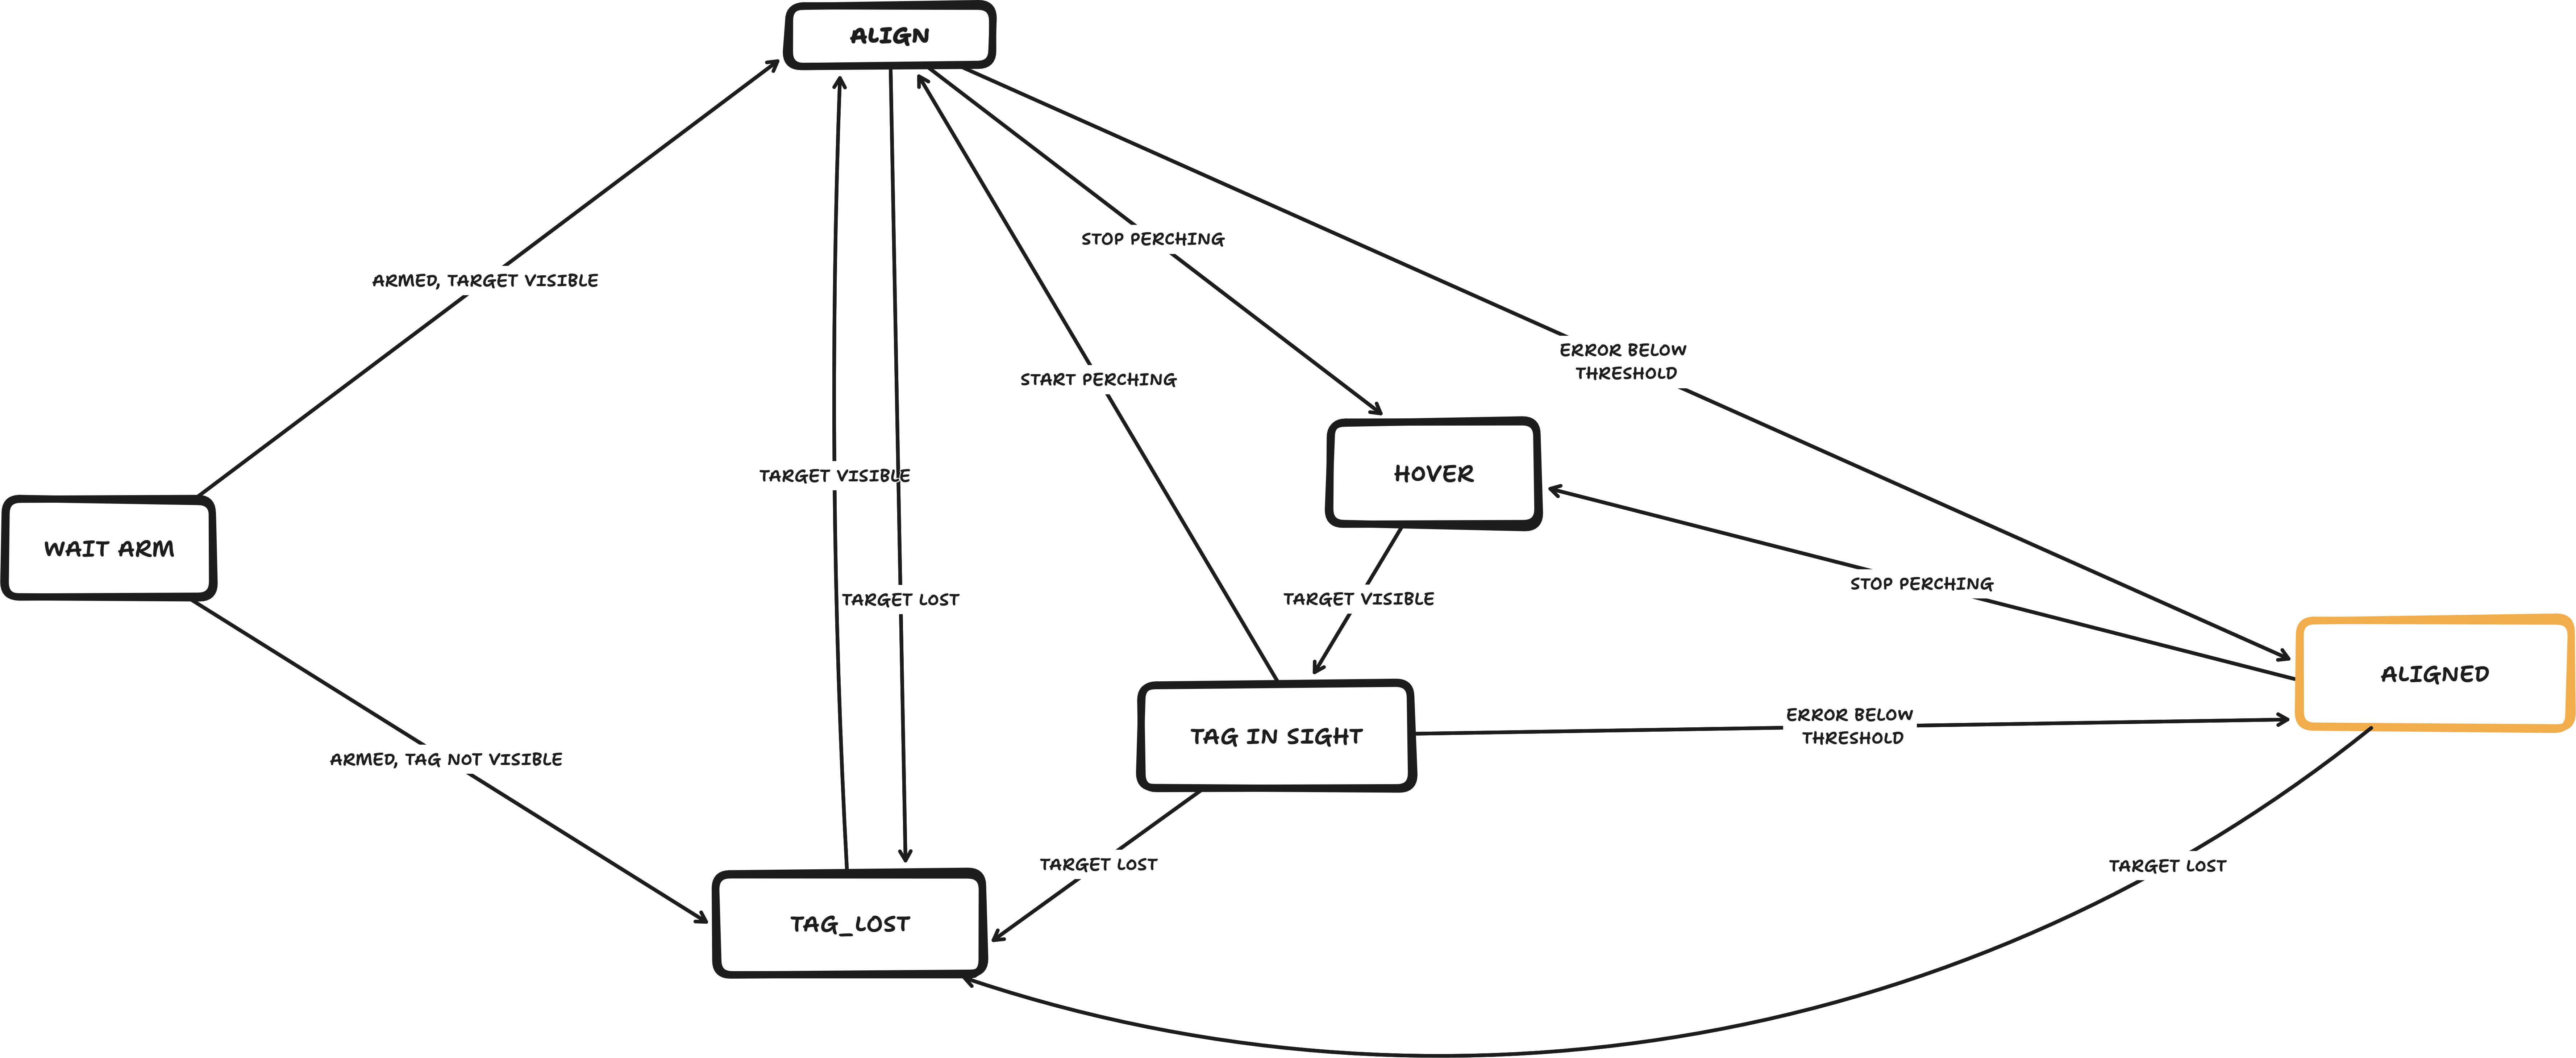
\includegraphics[width=1.0\textwidth]{images/state_machine.png}
\caption{Automat stanja upravljačkog sloja: sedam stanja i prijelazi između njih.}
\label{fig:state_machine}
\end{figure}

\subsection{Prilazak bez okidača temeljenog na mjerenju udaljenosti}
\label{subsec:prijanjanje}

Budući da senzor udaljenosti nije dostupan za okidanje manevra prijanjanja, vertikalno kretanje ne temelji se na izravnom mjerenju udaljenosti niti na bilo kojoj vrijednosti proslijeđenoj iz percepcijskog cjevovoda. Umjesto toga, upravljački sloj \texttt{ibvs\_perching} naredbu penjanja izvodi kao unaprijed zadanu konstantu (\texttt{perch\_climb\_thrust}), aktivnu u oba stanja poravnanja (poravnanje i poravnano, vidi Odjeljak~\ref{subsec:state-machine}) sve dok je bočna udaljenost detekcije od ciljne točke unutar zasebnog, šireg praga (\texttt{descend\_xy\_gate\_px}). Ta se udaljenost računa izravno iz sirove pikselne pogreške, neovisno o unutarnjoj normalizaciji regulacijske petlje, kako bi prag imao isto značenje bez obzira na to kako je regulator prethodno skalirao pogrešku. Time se izbjegava potreba za diskretnim okidačem temeljenim na mjerenju udaljenosti: penjanje se odvija kontinuirano dok je letjelica dovoljno bočno poravnata, umjesto da ga pokreće poseban signal iz percepcije ili zadržavanje u pojedinom stanju. Prag za penjanje namjerno je postavljen tako da nikad ne bude uži od praga koji definira ulazak u stanje poravnano, čime je osigurano da dosezanje stanja poravnano uvijek dopušta i penjanje. Penjanje ili spuštanje izvan tog praga izgurnulo bi granu iz vidnog polja kamere brže nego što bi je bočno poravnanje moglo ponovno uhvatiti.
